

%% This file was auto-generated by IPython.
%% Conversion from the original notebook file:
%%
\documentclass[11pt,english]{article}

%% This is the automatic preamble used by IPython.  Note that it does *not*
%% include a documentclass declaration, that is added at runtime to the overall
%% document.

\usepackage{amsmath}
\usepackage{amssymb}
\usepackage{graphicx}
\usepackage{grffile}
\usepackage{ucs}
\usepackage[utf8x]{inputenc}

% Scale down larger images
\usepackage[export]{adjustbox}

%fancy verbatim
\usepackage{fancyvrb}
% needed for markdown enumerations to work
\usepackage{enumerate}

% Slightly bigger margins than the latex defaults
\usepackage{geometry}
\geometry{verbose,tmargin=3cm,bmargin=3cm,lmargin=2.5cm,rmargin=2.5cm}

% Define a few colors for use in code, links and cell shading
\usepackage{color}
\definecolor{orange}{cmyk}{0,0.4,0.8,0.2}
\definecolor{darkorange}{rgb}{.71,0.21,0.01}
\definecolor{darkgreen}{rgb}{.12,.54,.11}
\definecolor{myteal}{rgb}{.26, .44, .56}
\definecolor{gray}{gray}{0.45}
\definecolor{lightgray}{gray}{.95}
\definecolor{mediumgray}{gray}{.8}
\definecolor{inputbackground}{rgb}{.95, .95, .85}
\definecolor{outputbackground}{rgb}{.95, .95, .95}
\definecolor{traceback}{rgb}{1, .95, .95}

% new ansi colors
\definecolor{brown}{rgb}{0.54,0.27,0.07}
\definecolor{purple}{rgb}{0.5,0.0,0.5}
\definecolor{darkgray}{gray}{0.25}
\definecolor{lightred}{rgb}{1.0,0.39,0.28}
\definecolor{lightgreen}{rgb}{0.48,0.99,0.0}
\definecolor{lightblue}{rgb}{0.53,0.81,0.92}
\definecolor{lightpurple}{rgb}{0.87,0.63,0.87}
\definecolor{lightcyan}{rgb}{0.5,1.0,0.83}

% Framed environments for code cells (inputs, outputs, errors, ...).  The
% various uses of \unskip (or not) at the end were fine-tuned by hand, so don't
% randomly change them unless you're sure of the effect it will have.
\usepackage{framed}

% remove extraneous vertical space in boxes
\setlength\fboxsep{0pt}

% codecell is the whole input+output set of blocks that a Code cell can
% generate.

% TODO: unfortunately, it seems that using a framed codecell environment breaks
% the ability of the frames inside of it to be broken across pages.  This
% causes at least the problem of having lots of empty space at the bottom of
% pages as new frames are moved to the next page, and if a single frame is too
% long to fit on a page, will completely stop latex from compiling the
% document.  So unless we figure out a solution to this, we'll have to instead
% leave the codecell env. as empty.  I'm keeping the original codecell
% definition here (a thin vertical bar) for reference, in case we find a
% solution to the page break issue.

%% \newenvironment{codecell}{%
%%     \def\FrameCommand{\color{mediumgray} \vrule width 1pt \hspace{5pt}}%
%%    \MakeFramed{\vspace{-0.5em}}}
%%  {\unskip\endMakeFramed}

% For now, make this a no-op...
\newenvironment{codecell}{}

 \newenvironment{codeinput}{%
   \def\FrameCommand{\colorbox{inputbackground}}%
   \MakeFramed{\advance\hsize-\width \FrameRestore}}
 {\unskip\endMakeFramed}

\newenvironment{codeoutput}{%
   \def\FrameCommand{\colorbox{outputbackground}}%
   \vspace{-1.4em}
   \MakeFramed{\advance\hsize-\width \FrameRestore}}
 {\unskip\medskip\endMakeFramed}

\newenvironment{traceback}{%
   \def\FrameCommand{\colorbox{traceback}}%
   \MakeFramed{\advance\hsize-\width \FrameRestore}}
 {\endMakeFramed}

% Use and configure listings package for nicely formatted code
\usepackage{listingsutf8}
\lstset{
  language=python,
  inputencoding=utf8x,
  extendedchars=\true,
  aboveskip=\smallskipamount,
  belowskip=\smallskipamount,
  xleftmargin=2mm,
  breaklines=true,
  basicstyle=\small \ttfamily,
  showstringspaces=false,
  keywordstyle=\color{blue}\bfseries,
  commentstyle=\color{myteal},
  stringstyle=\color{darkgreen},
  identifierstyle=\color{darkorange},
  columns=fullflexible,  % tighter character kerning, like verb
}

% The hyperref package gives us a pdf with properly built
% internal navigation ('pdf bookmarks' for the table of contents,
% internal cross-reference links, web links for URLs, etc.)
\usepackage{hyperref}
\hypersetup{
  breaklinks=true,  % so long urls are correctly broken across lines
  colorlinks=true,
  urlcolor=blue,
  linkcolor=darkorange,
  citecolor=darkgreen,
  }

% hardcode size of all verbatim environments to be a bit smaller
\makeatletter 
\g@addto@macro\@verbatim\small\topsep=0.5em\partopsep=0pt
\makeatother 

% Prevent overflowing lines due to urls and other hard-to-break entities.
\sloppy




\begin{document}



\begin{codecell}


\begin{codeinput}
\begin{lstlisting}
<style type="text/css">
.time_spent {
    width: 3em;
    border-style: none;
    background-color: silver;
    font-weight: bold;
    padding-left: 5px;
}
</style>
\end{lstlisting}
\end{codeinput}

\end{codecell}
\section{{[}WS13/14{]} Mathematics for Robotics and Control Assignment
003 - Matrix Decomposition}


\begin{codecell}


\begin{codeinput}
\begin{lstlisting}
import IPython.core.display
import sys
if not "win" in sys.platform and not "linux" in sys.platform:
    %pylab
else:
    %pylab inline
\end{lstlisting}
\end{codeinput}
\begin{codeoutput}


\begin{Verbatim}[commandchars=\\\{\}]
Populating the interactive namespace from numpy and matplotlib
\end{Verbatim}

\end{codeoutput}

\end{codecell}

\begin{center}\rule{3in}{0.4pt}\end{center}

\subsubsection{Function and Module List}


Each week, the assignment sheet will contain a list of Python modules
and functions you are supposed to know. These modules and functions will
help you to solve the assignments and many of them are required in later
assignments. You are expected to familiarize yourself with each module /
function listed here and to know when and how to apply them. Remember
this is especially important in the exam!

\textbf{Modules}:

\begin{itemize}
\item
  numpy.linalg
\end{itemize}
\textbf{Functions}:

numpy.linalg:

\begin{itemize}
\item
  qr, svd
\end{itemize}

\begin{center}\rule{3in}{0.4pt}\end{center}

\subsubsection{Assignment 3.1 {[}L1{]}}


Take the following matrix and obtain it's eigenvalues:

$A_0 = \begin{bmatrix}1.35264537e+00 & -2.83012728e-03 & 3.75980444e-01 \\ -2.83012728e-03 & 1.00491214e-02 & -2.40593554e-03\\ 3.75980444e-01 & -2.40593554e-03 & 4.51412148e+00\end{bmatrix}$

Now obtain the QR decomposition of $A_0$ and implement the following
algorithm:

\begin{enumerate}[1.]
\item
  $A_{k+1} = {Q_k^{-1}} \cdot A_k \cdot Q_k$
\end{enumerate}
\ldots{}and run it for at least 1500 iterations of $k$. What do you
notice about the resulting matrix $A_{1500}$?

\begin{codecell}


\begin{codeinput}
\begin{lstlisting}
# Solution 3.1
# ...


A = load('Matrix A.npy')

B = A.copy()
for i in xrange(1500):
    q, r = qr(B)
    B = dot(q.T, dot(B, q))

print eigvals(A)
print ' '
print B

print 'The diagonal is the eigenvals of A - the rest is almost zero'
#1h
\end{lstlisting}
\end{codeinput}
\begin{codeoutput}


\begin{Verbatim}[commandchars=\\\{\}]
[ 4.55822169  0.01004256  1.30855172]
 
[[  4.55822169e+000   1.58607411e-016  -2.20277079e-016]
 [ -4.94065646e-324   1.30855172e+000  -1.91014318e-016]
 [  4.94065646e-324   4.94065646e-324   1.00425639e-002]]
The diagonal is the eigenvals of A - the rest is almost zero
\end{Verbatim}

\end{codeoutput}

\end{codecell}

\emph{Assignment 3.1 took me} \emph{minutes.}

\begin{center}\rule{3in}{0.4pt}\end{center}

\subsubsection{Assignment 3.2 L1}


Watch the following video and write a summary about half a DINA4 page
long.

\begin{codecell}


\begin{codeinput}
\begin{lstlisting}
IPython.display.YouTubeVideo("OSGv2VnC0go")
\end{lstlisting}
\end{codeinput}
\begin{codeoutput}




\begin{verbatim}
<IPython.lib.display.YouTubeVideo at 0x31f6490>
\end{verbatim}



\end{codeoutput}

\end{codecell}

The talk ``Transforming Code into Beautiful, Idiomatic Python'' gives an
overview of how to write code in python. But it is not a basic tutorial,
but a list of common methods. For every method there is on obfuscated
code example, a person with C or Java background might come up with and
one clean and fast version how to do it in Python. Example functions to
use are: range, xrange, reversed, enumerate, izip and partial. Besides
these simple functions are more advanced concepts discussed. For example
the else in for loops, iteritems, named tuples, deque, @cache or ``with
ignored''. As a wrap-up, the speaker gives advice to use concise
expressive one-liners. That is to write the equivalent of one simple
sentence in one program statement.

\emph{Assignment 3.2 took me} \emph{minutes.}

\begin{center}\rule{3in}{0.4pt}\end{center}

\subsubsection{Assignment 3.3 L3}


Read \href{http://mathworld.wolfram.com/LeastSquaresFitting.html}{this
article about least squares fitting}. Read this
\href{http://classes.soe.ucsc.edu/cmps290c/Spring04/paps/lls.pdf}{paper
about linear least squares and matrix decompositions}. \textbf{For all
of the following fitting tasks, use a singular value decomposition to
fit a shape to each of the given point clouds. Show your results by
plotting bot the original points and the fitted shape. Determine what
kind of shape to use by inspecting the data points given to you. For
some tasks, you will have to use more than one shape (i.e.~fit two
parallel or orthogonal lines).}

\begin{codecell}


\begin{codeinput}
\begin{lstlisting}
# Solution 3.3
# ...

#SETUP
s1 = load('shape001.npy')
#roomcloud
#print s1.shape

s2 = load('shape0001.npy')
#split room cloud
#print s2.shape

s3 = load('shape002.npy')
#parallel lines
#print s3.shape

s4 = load('shape003.npy')
#orthogonal
#print s4.shape

\end{lstlisting}
\end{codeinput}

\end{codecell}

\begin{codecell}


\begin{codeinput}
\begin{lstlisting}
def line_fitting(A):
    #In the slides is A and B
    x = numpy.array(A[:, 0])
    y = A[:, 1] 
    
    X = numpy.matrix([numpy.ones(size(x)), x]).T
    Y = numpy.array([y]).T
    #print X[0]
    #print Y[0]
    
    #pinv = (AT*A)^(-1)*AT
    #pinv uses svd
    y_intercept, slope = dot(pinv(X), Y)
    
    x1 = x
    y1 = y
    for i in range(len(x)):
        y[i]=slope*x[i]+y_intercept
    
    line = numpy.matrix([x1, y1]).T
    #plot(x1[:], y1[:], 'x')
    
    return (line, slope, y_intercept)

##Show results
for cloud in [[s1], s2, s3, s4]:
    print '--New point cloud--'
    for l in cloud:
        plot(l[:,0], l[:, 1], 'o', alpha = 0.2)
        (line, slope, y_intercept) = line_fitting(l)
        plot(line[:,0], line[:,1])
        print 'Y='+str(slope)+'X+'+str(y_intercept)
    show()

#4h
\end{lstlisting}
\end{codeinput}
\begin{codeoutput}


\begin{Verbatim}[commandchars=\\\{\}]
--New point cloud--
Y=[[ 0.32360017]]X+[[ 5.11247047]]
\end{Verbatim}

\begin{center}
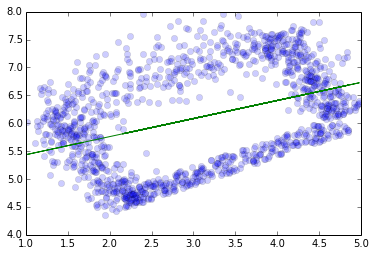
\includegraphics[max size={0.7\textwidth}{0.9\textheight}]{MRC_ChristopheQuignon_20140424_files/MRC_ChristopheQuignon_20140424_22_1.png}
\par
\end{center}

\begin{Verbatim}[commandchars=\\\{\}]
--New point cloud--
Y=[[ 0.50105763]]X+[[ 3.55896546]]
Y=[[-1.07109764]]X+[[ 11.54853522]]
Y=[[ 0.45613678]]X+[[ 5.72825777]]
\end{Verbatim}

\begin{center}
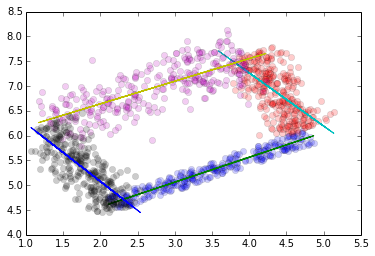
\includegraphics[max size={0.7\textwidth}{0.9\textheight}]{MRC_ChristopheQuignon_20140424_files/MRC_ChristopheQuignon_20140424_22_3.png}
\par
\end{center}

\begin{Verbatim}[commandchars=\\\{\}]
--New point cloud--
Y=[[ 1.80181864]]X+[[ 243.49120751]]
Y=[[ 1.7837933]]X+[[ 1.43905445]]
\end{Verbatim}

\begin{center}
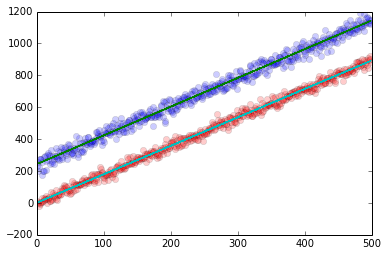
\includegraphics[max size={0.7\textwidth}{0.9\textheight}]{MRC_ChristopheQuignon_20140424_files/MRC_ChristopheQuignon_20140424_22_5.png}
\par
\end{center}

\begin{Verbatim}[commandchars=\\\{\}]
--New point cloud--
Y=[[ 2.33470863]]X+[[-177.64788787]]
Y=[[-2.33858783]]X+[[ 18.2858297]]
\end{Verbatim}

\begin{center}
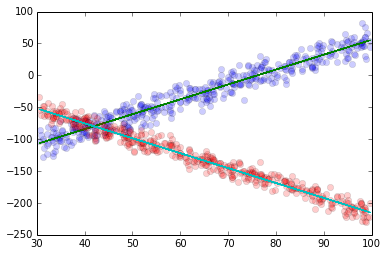
\includegraphics[max size={0.7\textwidth}{0.9\textheight}]{MRC_ChristopheQuignon_20140424_files/MRC_ChristopheQuignon_20140424_22_7.png}
\par
\end{center}

\end{codeoutput}

\end{codecell}

\emph{Assignment 3.3 took me} \emph{minutes.}

\begin{center}\rule{3in}{0.4pt}\end{center}


\emph{Use this button to create a .txt file containing the time in
minutes you spent working on the assignments. Make sure to include your
name in the textbox below. The file will be created in the current
directory.}

Student's name:



\end{document}

